\documentclass[11pt,a4paper]{article}
\usepackage{amsmath,amssymb,graphicx,booktabs,hyperref,siunitx}
\usepackage[margin=2.5cm]{geometry}
\graphicspath{{figures/}{../}}

\title{X2UHJ: From AmbiX to UHJ C-Format\\\large The Mathematics of the SEAM-LTM UHJ Plugin}
\author{Giuseppe Silvi --- SEAM}
\date{2026}

\begin{document}
\maketitle
\begin{abstract}
This document derives the mathematics of the \texttt{x2uhj} plugin step by step.
It covers the AmbiX-to-UHJ C-format encoding, the origin of Gerzon's matrix coefficients, and the sample-rate-independent design of the quadrature all-pass network.
\end{abstract}
\tableofcontents

\section{Introduction and Historical Framing}

UHJ is a hierarchical multichannel encoding system that represents a periphonic or horizontal sound field in a small number of channels suitable for stereo-compatible transmission and subsequent decoding.
The name ``UHJ'' derives from the BBC Matrix-H system and the 45J variant, both developed at the BBC in the 1970s as practical approaches to compatible surround sound.
Michael Gerzon unified and extended these systems in his 1985 AES paper, establishing the coefficient set that the \texttt{x2uhj} plugin implements.
The C-format variant carries four channels: the stereo pair $(L, R)$, a third directional channel $T$, and a height-related channel $Q$.

The \texttt{x2uhj} plugin accepts a First-Order AmbiX signal (four channels in ACN order, SN3D normalisation) and delivers UHJ C-format output.
This document derives Gerzon's matrix coefficients by inverse verification against known decoded loudspeaker positions.
It establishes the quadrature all-pass network as a sample-rate-independent design procedure, enabling consistent behaviour across all standard audio sample rates.

\section{AmbiX to FuMa}

The plugin first converts the incoming ACN/SN3D channels to the FuMa convention used throughout the UHJ literature.
ACN orders the four first-order channels as $A_0$ (omnidirectional), $A_1$ (front--back), $A_2$ (up--down), $A_3$ (left--right), corresponding to the spherical harmonic sequence $W, Y, Z, X$.
FuMa arranges the same signals as $W, X, Y, Z$ and scales the omnidirectional component by $1/\sqrt{2}$.
The conversion is therefore a reindexing together with a single rescaling:

\begin{equation}
W = \tfrac{1}{\sqrt{2}}\,A_0,\quad X = A_3,\quad Y = A_1,\quad Z = A_2 .
\end{equation}

All subsequent matrix operations in this document refer to the FuMa signals $W, X, Y, Z$.

\section{The UHJ C-Format Matrix}

Gerzon's UHJ encoding proceeds in two stages: formation of the intermediate sum and difference signals $\Sigma$ and $\Delta$, followed by the channel assignments for $L$, $R$, $T$, and $Q$.

\begin{align}
\Sigma &= 0.9396926\,W + 0.1855740\,X ,\\
\Delta &= j(-0.3420201\,W + 0.5098604\,X) + 0.6554516\,Y ,\\
L &= \tfrac{1}{2}(\Sigma + \Delta), \qquad R = \tfrac{1}{2}(\Sigma - \Delta),\\
T &= j(-0.1432\,W + 0.6512\,X) - 0.7071\,Y, \qquad Q = 0.9772\,Z .
\end{align}

$\Sigma$ is the forward-facing sum channel; its first-order pattern secures mono compatibility across all playback configurations.
$\Delta$ is the difference channel; the factor $j$ introduces a broadband 90-degree phase shift that encodes lateral width.
$L$ and $R$ are the two transmitted stereo channels, formed from the sum and difference of $\Sigma$ and $\Delta$.
$T$ is the third C-format channel; it carries additional directional resolution that extends spatial accuracy beyond the stereo base.
$Q$ is the height-related channel; it carries the vertical component $Z$ scaled by $0.9772$ to match the overall normalisation scheme.
The symbol $j$ denotes a broadband 90-degree phase shift applied across the full audio bandwidth; its implementation as a sample-rate-independent all-pass network is the subject of Sections~5 and~6.
\section{Reconstructing Gerzon's Coefficients}

Gerzon chose the UHJ coefficients to reproduce the psychoacoustic localization of the original sound field.
The velocity vector $\mathbf{r}_V$ governs perceived direction below roughly \SI{700}{\hertz}, and the energy vector $\mathbf{r}_E$ governs it above.
Both vectors are weighted averages of the loudspeaker direction unit vectors $\hat{\mathbf{u}}_i$:

\begin{equation}
\mathbf{r}_V = \frac{\sum_i g_i\,\hat{\mathbf{u}}_i}{\sum_i g_i},
\qquad
\mathbf{r}_E = \frac{\sum_i g_i^{2}\,\hat{\mathbf{u}}_i}{\sum_i g_i^{2}} .
\end{equation}

The velocity vector uses the loudspeaker gains $g_i$ directly, and the energy vector uses their squared values.
A well-designed encoding keeps both vectors pointing toward the original source azimuth, with magnitude near unity.

The constants in the $\Sigma$ and $\Delta$ expressions carry geometric meaning.
The coefficient $0.9396926 = \cos 20^\circ$ and $0.3420201 = \sin 20^\circ$ reveal the $20^\circ$ design angle that Gerzon selected to balance spatial precision and robust mono compatibility.
$\Sigma$ realises a forward first-order microphone pattern, which secures mono compatibility across all playback configurations.
The $j$ term in $\Delta$ supplies the degree of freedom that maps the full \ang{360} of azimuth into two channels reversibly.

Inverse verification takes the published coefficients as given and confirms numerically that they realise good localization.
The verification evaluates two listening models.
The surround model feeds $(L, R)$ to a symmetric illustrative loudspeaker layout and reads the localization vectors of the reconstructed field.
The super-stereo model feeds $(L, R)$ to two frontal loudspeakers at \ang{30} and \ang{-30} and reads the localization a listener perceives at those positions.

\begin{figure}[h]\centering
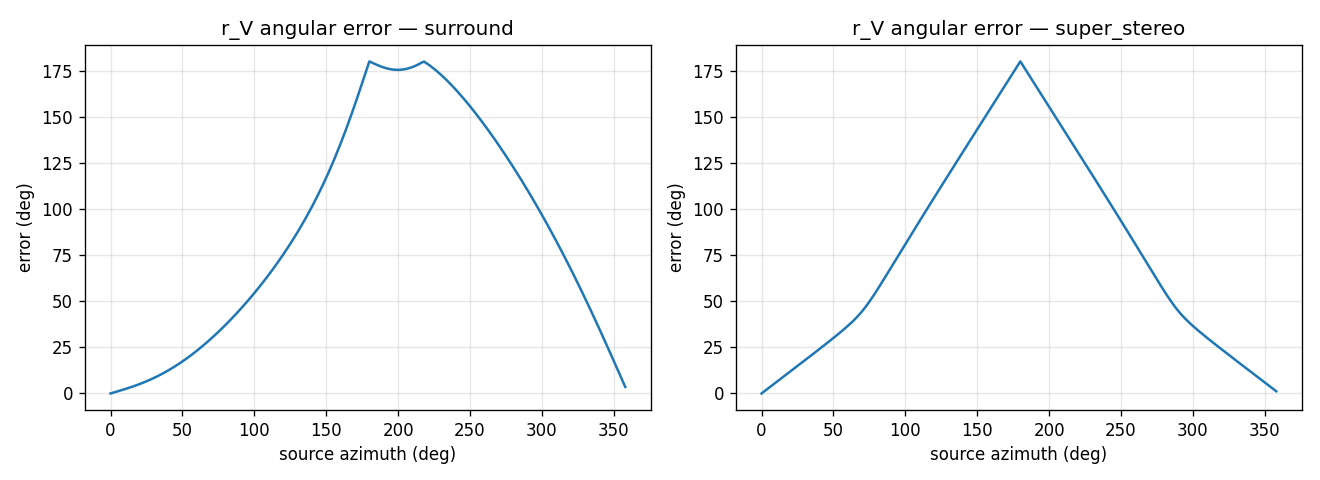
\includegraphics[width=\linewidth]{gerzon_localization.png}
\caption{Velocity-vector angular error versus source azimuth: surround decode (left) and super-stereo (right). Both models confirm that Gerzon's published coefficients localise the source across azimuth.}
\end{figure}

The surround model illuminates why Gerzon selected these coefficients: the reconstructed field localises faithfully across the full azimuth circle.
The super-stereo model demonstrates the stereo listening result: a frontal pair at $\pm30^\circ$ conveys the same source direction with small angular error.
Agreement between the two models across azimuth confirms that the published coefficients serve both listening contexts.
\section{The \texorpdfstring{$j$}{j} Problem: Wideband 90 Degrees}

The $j$ operator in the UHJ matrix denotes a 90-degree phase shift applied uniformly across the audio band.
A broadband 90-degree phase difference between two filter paths realises this operator.
A FIR Hilbert pair achieves the phase difference with a tap set fixed to one sample rate and one length.
An IIR all-pass pair carries the same phase relation in physical $(f_0, Q)$ units, which expresses the design in sample-rate-free terms.
This section develops the IIR all-pass approach and establishes the procedure that holds the quadrature at every sample rate.

\section{The Sample-Rate-Independent Design}

The analog second-order all-pass prototype and its phase response are:

\begin{equation}
H_a(s) = \frac{s^2 - (\omega_0/Q)\,s + \omega_0^2}{s^2 + (\omega_0/Q)\,s + \omega_0^2},
\qquad \omega_0 = 2\pi f_0 .
\end{equation}

\begin{equation}
\varphi_a(\omega) = -2\arctan\!\frac{(\omega_0/Q)\,\omega}{\omega_0^2 - \omega^2} .
\end{equation}

Each network is a cascade of three second-order all-pass sections, one for the real path $H_R$ and one for the imaginary path $H_I$.
Optimising the six $(f_0, Q)$ pairs so that $\varphi_{H_I} - \varphi_{H_R} = -\ang{90}$ over \SIrange{20}{20000}{\hertz} on the analog phase reaches a maximum error of \ang{0.40} in the continuous domain.

\begin{table}[h]
\centering
\caption{Analog $s$-domain ideal $(f_0, Q)$ pairs. Maximum phase error \ang{0.40} across \SIrange{20}{20000}{\hertz}.}
\label{tab:analog-pairs}
\begin{tabular}{@{}lcc@{}}
\toprule
Path & $f_0$ (Hz) & $Q$ \\
\midrule
$H_R$ & 107.988  & 0.2267 \\
$H_R$ & 449.085  & 0.2406 \\
$H_R$ & 19474.604 & 0.3194 \\
\addlinespace
$H_I$ & 20.540   & 0.3194 \\
$H_I$ & 1756.151 & 0.4026 \\
$H_I$ & 1878.679 & 0.1198 \\
\bottomrule
\end{tabular}
\end{table}

The RBJ bilinear realisation maps each analog section to a digital biquad all-pass:

\begin{equation}
a_1 = \frac{-2\cos\omega}{1+\alpha},\quad a_2 = \frac{1-\alpha}{1+\alpha},\quad
\alpha = \frac{\sin\omega}{2Q},\quad \omega = \frac{2\pi f_0}{f_s},
\end{equation}

with all-pass numerator $b = [a_2,\, a_1,\, 1]$.

The bilinear transform maps a digital frequency $f$ to the analog frequency $F = (f_s/\pi)\tan(\pi f / f_s)$.
A fixed $(f_0, Q)$ set therefore presents its broadband phase on a warped frequency axis that depends on $f_s$.
The quadrature holds near the sample rate the set was designed for, and the phase difference departs from \ang{90} as the sample rate moves away.
Sample-rate independence belongs to the design procedure: re-running the digital phase fit at the actual sample rate restores the quadrature at that rate.
The deliverable stores a per-rate $(f_0, Q)$ table, with one entry produced by the same procedure for each standard rate.

\begin{table}[h]
\centering
\caption{Per-rate design maxima. Each row is designed independently at its own sample rate.}
\label{tab:per-rate}
\begin{tabular}{@{}cc@{}}
\toprule
Sample rate (kHz) & Max phase error (deg) \\
\midrule
44.1  & 2.040 \\
48    & 1.362 \\
88.2  & 0.529 \\
96    & 0.505 \\
176.4 & 0.429 \\
192   & 0.425 \\
\bottomrule
\end{tabular}
\end{table}

The per-rate table holds the quadrature within roughly two degrees at every standard rate.
Section~7 visualises this against the phase drift of a fixed set applied across varying sample rates.
% \section{Validation}                             % Task 11
% \section*{References}                            % Task 11

\bibliographystyle{IEEEtran}
\bibliography{refs}
\end{document}
